\documentclass{report}
\usepackage[utf8]{inputenc}
\usepackage[english, russian]{babel}
\usepackage{listings}
\usepackage{graphicx}
\usepackage{amsmath,amsfonts,amssymb,amsthm,mathtools} 
\usepackage{pgfplots}
\usepackage{filecontents}
\usepackage{indentfirst}
\usepackage{eucal}
\usepackage{enumitem}
\frenchspacing

\usepackage{indentfirst} % Красная строка

\usetikzlibrary{datavisualization}
\usetikzlibrary{datavisualization.formats.functions}

\usepackage{amsmath}



% Для листинга кода:
\lstset{ %
language=c++,                 % выбор языка для подсветки (здесь это С)
basicstyle=\small\sffamily, % размер и начертание шрифта для подсветки кода
numbers=left,               % где поставить нумерацию строк (слева\справа)
numberstyle=\tiny,           % размер шрифта для номеров строк
stepnumber=1,                   % размер шага между двумя номерами строк
numbersep=5pt,                % как далеко отстоят номера строк от подсвечиваемого кода
showspaces=false,            % показывать или нет пробелы специальными отступами
showstringspaces=false,      % показывать или нет пробелы в строках
showtabs=false,             % показывать или нет табуляцию в строках
frame=single,              % рисовать рамку вокруг кода
tabsize=2,                 % размер табуляции по умолчанию равен 2 пробелам
captionpos=t,              % позиция заголовка вверху [t] или внизу [b] 
breaklines=true,           % автоматически переносить строки (да\нет)
breakatwhitespace=false, % переносить строки только если есть пробел
escapeinside={\#*}{*)}   % если нужно добавить комментарии в коде
}

\usepackage[left=2cm,right=2cm, top=2cm,bottom=2cm,bindingoffset=0cm]{geometry}
% Для измененных титулов глав:
\usepackage{titlesec, blindtext, color} % подключаем нужные пакеты
\definecolor{gray75}{gray}{0.75} % определяем цвет
\newcommand{\hsp}{\hspace{20pt}} % длина линии в 20pt
% titleformat определяет стиль
\titleformat{\chapter}[hang]{\Huge\bfseries}{\thechapter\hsp\textcolor{gray75}{|}\hsp}{0pt}{\Huge\bfseries}


% plot
\usepackage{pgfplots}
\usepackage{filecontents}
\usetikzlibrary{datavisualization}
\usetikzlibrary{datavisualization.formats.functions}
 
\begin{document}
  %\def\chaptername{} % убирает "Глава"
\thispagestyle{empty}
\begin{titlepage}
	\noindent \begin{minipage}{0.15\textwidth}
	
\includegraphics[width=\linewidth]{b_logo}
	\end{minipage}
	\noindent\begin{minipage}{0.9\textwidth}\centering
		\textbf{Министерство науки и высшего образования Российской Федерации}\\
		\textbf{Федеральное государственное бюджетное образовательное учреждение высшего образования}\\
		\textbf{~~~«Московский государственный технический университет имени Н.Э.~Баумана}\\
		\textbf{(национальный исследовательский университет)»}\\
		\textbf{(МГТУ им. Н.Э.~Баумана)}
	\end{minipage}
	
	\noindent\rule{18cm}{3pt}
	\newline\newline
	\noindent ФАКУЛЬТЕТ $\underline{\text{«Информатика и системы управления»}}$ \newline\newline
	\noindent КАФЕДРА $\underline{\text{«Программное обеспечение ЭВМ и информационные технологии»}}$\newline\newline\newline\newline\newline\newline\newline\newline\newline\newline\newline
	
	
	\begin{center}
		\noindent\begin{minipage}{1.3\textwidth}\centering
			\Large\textbf{  Отчет по лабораторной работе №3}\newline
			\textbf{по дисциплине "Анализ алгоритмов"}\newline\newline
		\end{minipage}
	\end{center}
	
	\noindent\textbf{Тема} $\underline{\text{Алгоритмы сортировки}}$\newline\newline
	\noindent\textbf{Студент} $\underline{\text{Варламова Е. А.}}$\newline\newline
	\noindent\textbf{Группа} $\underline{\text{ИУ7-51Б}}$\newline\newline
	\noindent\textbf{Оценка (баллы)} $\underline{\text{~~~~~~~~~~~~~~~~~~~~~~~~~~~}}$\newline\newline
	\noindent\textbf{Преподаватель: } $\underline{\text{Волкова Л.Л.}}$\newline\newline\newline
	
	\begin{center}
		\vfill
		Москва~---~\the\year
		~г.
	\end{center}
\end{titlepage}


\tableofcontents
  
\newpage
\chapter*{Введение}
\addcontentsline{toc}{chapter}{Введение}


Сортировка является очень важной задачей обработки информации. При этом под сортировкой понимают процесс упорядочивания элементов по какому-либо признаку в заданном массиве объектов. Например, текстовые данные можно отсортировать в лексикографическом порядке, а числовые в порядке неубывания или невозрастания.

В настоящее время многие программные системы работают с большим объёмом данных, поэтому возникает задача ускорения процесса обработки. Именно эту задачу и решают алгоритмы сортировки. Так, время поиска в отсортированном массиве пропорционально логарифму количества элементов, а в неотсортированном - пропорционально количеству элементов, что значительно медленнее.

Важной характеристикой любого алгоритма сортировки является скорость его работы, то есть время, за которое данные будут отсортированы. Время сортировки будет зависеть от количества сравнений и перестановок элементов, а также от длины массива данных. 

Поэтому \textbf{целью} данной работы является получить навыки сравнительного анализа на примере 3 алгоритмов сортировки: сортировки пузырьком, сортировки выбором и быстрой сортировки. 

Для достижения поставленной цели необходимо решить следующие \textbf{задачи}:
\begin{itemize}
\item изучить алгоритмы сортировки;
\item провести сравнительный анализ алгоритмов на основе теоретических расчётов;
\item реализовать алгоритмы сортировки;
\item протестировать реализованные алгоритмы;
\item провести сравнительный анализ реализаций алгоритмов по затраченному процессорному времени.
\end{itemize}


\chapter{Аналитическая часть}

\section{Сортировка пузырьком}

Идея алгоритма состоит в последовательных проходах по массиву. За один проход элементы всех пар стоящих рядом элементов сравнивают друг с другом и, если они стоят в неправильном порядке, меняют их местами. Проходы повторяются N-1 раз, где N - длина массива. Доказывается, что такое количество проходов достаточно для получения отсортированного массива. Действительно, при сортировке чисел по возрастанию за первый проход ``выплывает'' на последнее место наибольший элемент. Так, за один проход, как минимум, один элемент встаёт на правильное место. Поэтому после N-1 проходов все элементы будут на своих местах. 

Из описания алгоритма очевидна модификация, ускоряющая его: если за проход не было обменов, то все элементы стоят на своих местах, следовательно, можно закончить выполнение сортировки. 

При этом важно заметить, что алгоритм является устойчивым, то есть одинаковые по заданному признаку элементы останутся в том же порядке, что и до сортировки.

\section{Сортировка выбором}

Идея алгоритма состоит в том, что массив делят на 2 части: отсортированную и неотсортированную. Части отделяет текущий элемент. Текущий элемент сравнивают с каждым элементом из неотсортированной части. Если элементы стоят в неправильном порядке, то запоминают элемент из неотсортированной части и его позицию. Далее сравнивают уже запомненный элемент и элементы из неотсортированной части. Так продолжается до конца массива. Эти действия напоминают поиск минимума (максимума) в числовом массиве. В результате одного такого прохода получают позицию некоторого элемента. Если эта позиция не совпадает с позицией текущего элемента, то элементы меняют местами, иначе ничего не происходит. Такущий элемент помечается как граница отсортированной части, а текущим назначается следующий элемент. Алгоритм заканчивается тогда, когда отсортированной частью массива будет являться весь массив. 

Важно заметить, что алгоритм не является устойчивым.

\section{Быстрая сортировка}

Идея алгоритма состоит в следующем:

\begin{itemize}
	\item выбрать из массива элемент, называемый опорным. Это может быть любой из элементов массива. От выбора опорного элемента не зависит корректность алгоритма, но может зависеть его эффективность. Обычно выбирают средний элемент.
	\item сравнить все остальные элементы с опорным и переставить их в массиве так, чтобы разбить массив на два отрезка: «меньшие опорного» и «равные и большие».
	\item для двух отрезков рекурсивно применяем ту же последовательность действий, пока длина отрезка больше единицы.
\end{itemize}

\section{Вывод}

В данном разделе были описаны идеи трёх алгоритмов сортировки: сортировки пузырьком, сортировки выбором и быстрой сортировки.
	
\clearpage

\chapter{Конструкторская часть}

\section{Схемы алгоритмов}

На рисунках 2.1, 2.2 и 2.3 показаны схемы алгоритмов сортировки пузырьком, выбором и быстрой сортировки соответственно.

\begin{figure}[h!p]
	\centering
	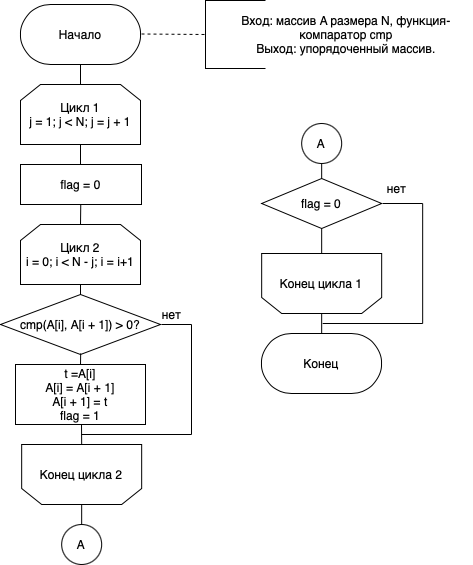
\includegraphics[scale = 0.75]{bsort.png}
	\caption{Схема сортировки пузырьком}
	\label{fig:mpr}
\end{figure}

\begin{figure}[h!p]
	\centering
	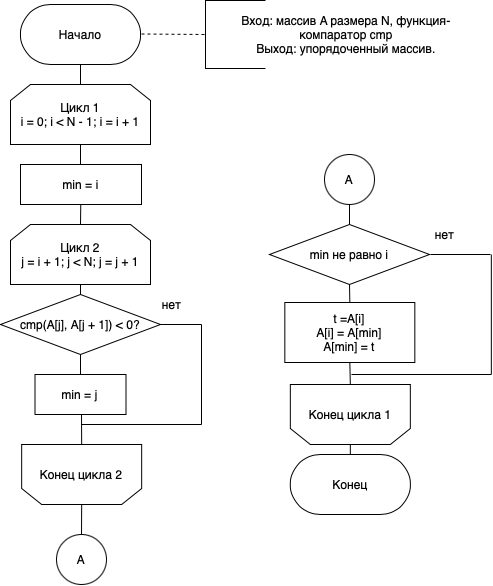
\includegraphics[width=0.9\linewidth]{ssort.png}
	\caption{Схема сортировки выбором}
	\label{fig:mpr}
\end{figure}

\begin{figure}[h!p]
	\centering
	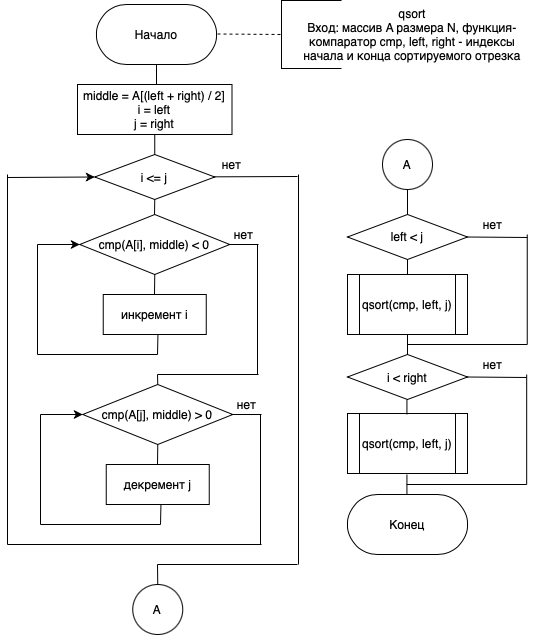
\includegraphics[width=1\linewidth]{qsort.png}
	\caption{Схема быстрой сортировки}
	\label{fig:mpr}
\end{figure}


\section{Трудоемкость алгоритмов}
Введем модель трудоемкости для оценки алгоритмов:
\begin{enumerate}
  	\item  базовые операции стоимостью 1 — +, -, *, /, =, ==, <=, >=, !=, +=, [], получение полей класса
	\item оценка трудоемкости цикла: Fц = a + N*(a + Fтела), где a - условие цикла
	\item стоимость условного перехода возьмем за 0, стоимость вычисления условия остаётся.
\end{enumerate}

Далее будет приведены оценки трудоемкости алгоритмов. Построчная оценка трудоемкости сортировки пузырькм с флагом (Табл. 2.1) и построчная оценка трудоемкости сортировки выбором (Табл. 2.2).

\subsection{Сортировка пузырьком с флагом}
\begin{center}
Табл. 2.1 Построчная оценка веса
	\begin{tabular}{|l c|} 
 	\hline
	Код & Вес \\ [0.5ex] 
 	\hline
	bool flag = false; & 1\\
	\hline
	int j = 1; & 1\\
 	\hline
	while (j < length) & 1\\
	\hline
	\{ & 0\\
	\hline
	flag = false; & 1\\
	\hline
	int i = 0; & 1\\
 	\hline
	while (i < length - j) & 2\\
	\hline
	\{ & 0\\	
	\hline
	if(cmp(arr[i], arr[i + 1]) > 0) & 4\\
	\hline
	\{ & 0\\
	\hline
	tmp = arr[i]; & 2\\
	\hline
    arr[i] = arr[i + 1]; & 3\\
    \hline
    arr[i + 1] = tmp; & 2\\
    \hline
    flag = true; & 1\\
    \hline
    \} & 0\\
	\hline
	i++; & 1\\
	\hline
	\} & 0\\
	\hline
	if (flag == false) break;  & 1\\
	\hline
	j++; & 1\\
	\hline
	\} & 0\\
	\hline
	\end{tabular}
\end{center}

 
\textbf{Лучший случай:} Массив отсортирован; не произошло ни одного обмена за 1 проход -> выходим из цикла \newline
Трудоемкость:  $1 + 1 + 1 + 1 * (1 + 1 + 2 + (n - 1) * (2 + 4 + 1) + 1) = 8 * n = O(n)$

\textbf{Худший случай:}  Массив отсортирован в обратном порядке; в каждом случае происходил обмен, все внутренние циклы будут состоять из N - j итераций.\newline
Трудоемкость: 
\newline
Внутренний цикл: $(n - 1) * (n - 2) * (2 + 4 + 2 + 3 + 2 + 1 + 1) / 2 = (n^2 -3n + 3) * 15 / 2 = 7.5n^2 - 22.5n + 22.5$
\newline
Внешний цикл: $1 + 1 + 1 + (n - 1) * (1 + 1 + 1 + 2 + 1 + 1) = 7n - 4$
\newline
Итог: $7.5 n^2 - 22.5n + 22.5 + 7n - 4 = 7.5n^2 - 15.5n + 18.5 = O(n ^ 2)$


\subsection{Сортировка выбором}
\begin{center}
Табл. 2.2 Построчная оценка веса
	\begin{tabular}{|l c|} 
 	\hline
	Код & Вес \\ [0.5ex] 
 	\hline
	int i = 0; & 1\\
 	\hline
	while (i < length - 1) & 2\\
	\hline
	\{ & 0\\
	\hline
	min = i; & 1\\
	\hline
	int j = i + 1; & 2\\
 	\hline
	while (j < length ) & 1\\
	\hline
	\{ & 0\\	
	\hline
	if(cmp(arr[j], arr[min]) < 0) & 4\\
	\hline
	\{ & 0\\
    \hline
    min = j; & 1\\
    \hline
    \} & 0\\
	\hline
	j++; & 1\\
	\hline
	\} & 0\\
	\hline
	if (min != i) & 1\\
	\hline
	\{ & 0\\
	\hline
	tmp = arr[i]; & 2\\
	\hline
    arr[i] = arr[min]; & 2\\
    \hline
    arr[min] = tmp; & 2\\
    \hline
	\} & 0\\
	\hline
	i++; & 1\\
	\hline
	\} & 0\\
	\hline
	\end{tabular}
\end{center}
\hspace*{5mm}
\textbf{Лучший случай:} отсортированный массив, обмены не производятся.
\newline
Трудоемкость: 
\newline
Внешний цикл: $1 + 2 + (n - 1) * (2 + 1 + 2 + 1 + 1) = 7n - 4$
\newline
Внутренний цикл: $(n - 1) * (n - 2) * (1 + 4 + 1) / 2 = 3n^2 -9n -9$
\newline
Итог: $3n^2 -9n -9 + 7n - 4 = 3n^2 -2n - 11 = O(n^2)$
\newline
\hspace*{5mm}
\textbf{Худший случай:} массив отсортирован в обратном порядке, все обмены будут произведены. \newline
Трудоемкость: 
\newline
Внешний цикл: $1 + 2 + (n - 1) * (2 + 1 + 2 + 1 + 2 + 2 + 2 + 1) = 13n - 10$
\newline
Внутренний цикл: $(n - 1) * (n - 2) * (1 + 4 + 1 + 1) / 2 = 3.5n^2 -10.5n -10.5$
\newline
Итог: $3.5n^2 -10.5n -10.5 + 13n - 10 = 3.5n^2 -2.5n - 20.5 = O(n^2)$

\subsection{Быстрая сортировка}
\textbf{Лучший случай:} сбалансированное дерево вызовов \(O(n*log(n))\). 
В cбалансированном варианте при каждой операции разделения массив делится на две одинаковые части, следовательно, максимальная глубина рекурсии, при которой размеры обрабатываемых подмассивов достигнут 1, составит log2n. В результате количество сравнений, совершаемых быстрой сортировкой, равно значению рекурсивного выражения $C_n = 2 * C_{n / 2} + n$, что дает общую сложность O(nlogn) [1].

\textbf{Худший случай:} несбалансированное дерево $O(n^2)$.
В несбалансированном варианте каждое разделение даёт два подмассива размерами 1 и n − 1, то есть при каждом рекурсивном вызове больший массив будет на 1 короче, чем в предыдущий раз. В этом случае потребуется $\sum_{{i=0}}^{n}(n-i)=O(n^{2})$ операций, то есть сортировка будет выполняться за квадратичное время [1].
\section{Вывод}
На основе описания алгоритмов, данного в аналитическом разделе, были построены схемы трёх алгоритмов сортировки, оценены их трудёмкости в лучшем и худшем случаях. Таким образом:
\begin{itemize}
\item сортировка пузырьком: лучший - $O(n)$, худший - $O(n^2)$ 
\item сортировка выбором: лучший - $O(n^2)$, худший - $O(n^2)$ 
\item быстрая сортировка: лучший - $O(nlogn)$, худший - $O(n^2)$ 
\end{itemize}
\chapter{Технологическая часть}

\section{Средства реализации}

В качестве языка программирования был выбран C++, поскольку он является достаточно быстрым, а среды разработки -- CLion. Время работы алгоритмов было замерено с помощью clock() [2].

\section{Входные и выходные данные}
На вход ПО получает массив сравнимых элементов и функцию сравнения двух элементов. На выходе -- тот же массив, но отсортированный в заданном порядке.

\section{Реализация алгоритмов}

В листингах 3.1 - 3.3 приведена реализация трёх алгоритмов сортировки.

\begin{lstlisting}[label=some-code,caption=Функция быстрой сортировки,language=C++]
template <typename Type>
void Array<Type>::_qsort(int (*cmp)(Type, Type), int left, int right)
{
    Type middle = data[(right + left) / 2];

    int i = left;
    int j = right;

    while (i <= j)
    {
        while (cmp(data[i], middle) < 0)
            i++;
        while (cmp(data[j], middle) > 0)
            j--;

        if (i <= j)
        {
            Type tmp = data[i];
            data[i] = data[j];
            data[j] = tmp;
            i++;
            j--;
        }
    }
    if (left < j)
        _qsort(cmp, left, j);
    if (i < right)
        _qsort(cmp, i, right);
}
\end{lstlisting}

\begin{lstlisting}[label=some-code,caption=Функция сортировки массива пузырьком, language=C++]
template <typename Type>
void Array<Type>::bubble(int (*cmp)(Type, Type))
{
    bool fl;
    for (size_t j = 1; j < length; j++) {
        fl = false;
        for (size_t i = 0; i < length - j; i++) {
            if (cmp(data[i], data[i + 1]) > 0) {
                Type tmp = data[i];
                data[i] = data[i + 1];
                data[i + 1] = tmp;
                fl = true;
            }
        }
        if (!fl)
            break;
    }
}
\end{lstlisting}

\begin{lstlisting}[label=some-code,caption=Функция сортировки массива выбором,language=C++]
template <typename Type>
void Array<Type>::selection(int (*cmp)(Type, Type))
{
    for (size_t i = 0; i < length - 1; i++)
    {
        size_t min = i;
        for (size_t j = i + 1; j < length; j++)
        {
            if (cmp(data[j], data[min]) < 0)
            {
                min = j;
            }
        }
        if (min != i)
        {
            Type tmp = data[i];
            data[i] = data[min];
            data[min] = tmp;
        }
    }
}
\end{lstlisting}


\section{Тестирование}

В таблице~\ref{tbl:test} приведены тесты для функций, реализующих алгоритмы сортировки. Все тесты пройдены успешно.

\begin{table}[h!]
	\begin{center}
		\begin{tabular}{|c|c|c|}
			\hline
			Входной массив & Результат & Ожидаемый результат \\ 
			\hline
			$[-4, -4, -9, 9, 2]$ & $[-9, -4, -4, 2, 9]$  & $[-9, -4, -4, 2, 9]$\\\hline
			$[-5, 6, -1, 5, 8]$  & $[-5, -1, 5, 6, 8]$  & $[-5, -1, 5, 6, 8]$\\\hline
			$[7]$  & $[7]$  & $[7]$\\\hline
			$[7, 1, 5, 2, 10]$  & $[1, 2, 5, 7, 10]$  & $[1, 2, 5, 7, 10]$\\\hline
			$[1, 0]$  & $[0, 1]$  & $[0, 1]$\\\hline
		\end{tabular}
		\caption{\label{tbl:test}Тестирование реализованных алгоритмов}
	\end{center}
\end{table}

\section{Вывод}

В данном разделе были выбраны средства разработки и с помощью них реализованы три алгоритма сортировки: пузырьком, выбором и быстрая сортировка. Кроме того, было проведено тестирование реализованных алгоритмов.

\chapter{Исследовательская часть}

\section{Технические характеристики}

Ниже приведены технические характеристики устройства, на котором было проведено тестирование ПО:

\begin{itemize}
	\item Операционная система: macOS Big Sur 64-bit.
	\item Оперативная память: 8 GB.
	\item Процессор: 1,4 GHz 4‑ядерный процессор Intel Core i5.

\end{itemize}

\section{Время выполнения алгоритмов}
Процессорное время выполнения алгоритма замерялось с помощью clock()[2]: для более точного замера каждая сортировка на каждой длине массива считалась несколько раз, а затем время усреднялось. 
На рисунках 4.1, 4.2 и 4.3 показаны графики зависимости процессорного времени выполнения сортировок от размера массива.

\begin{figure}[h!p]
	\centering
	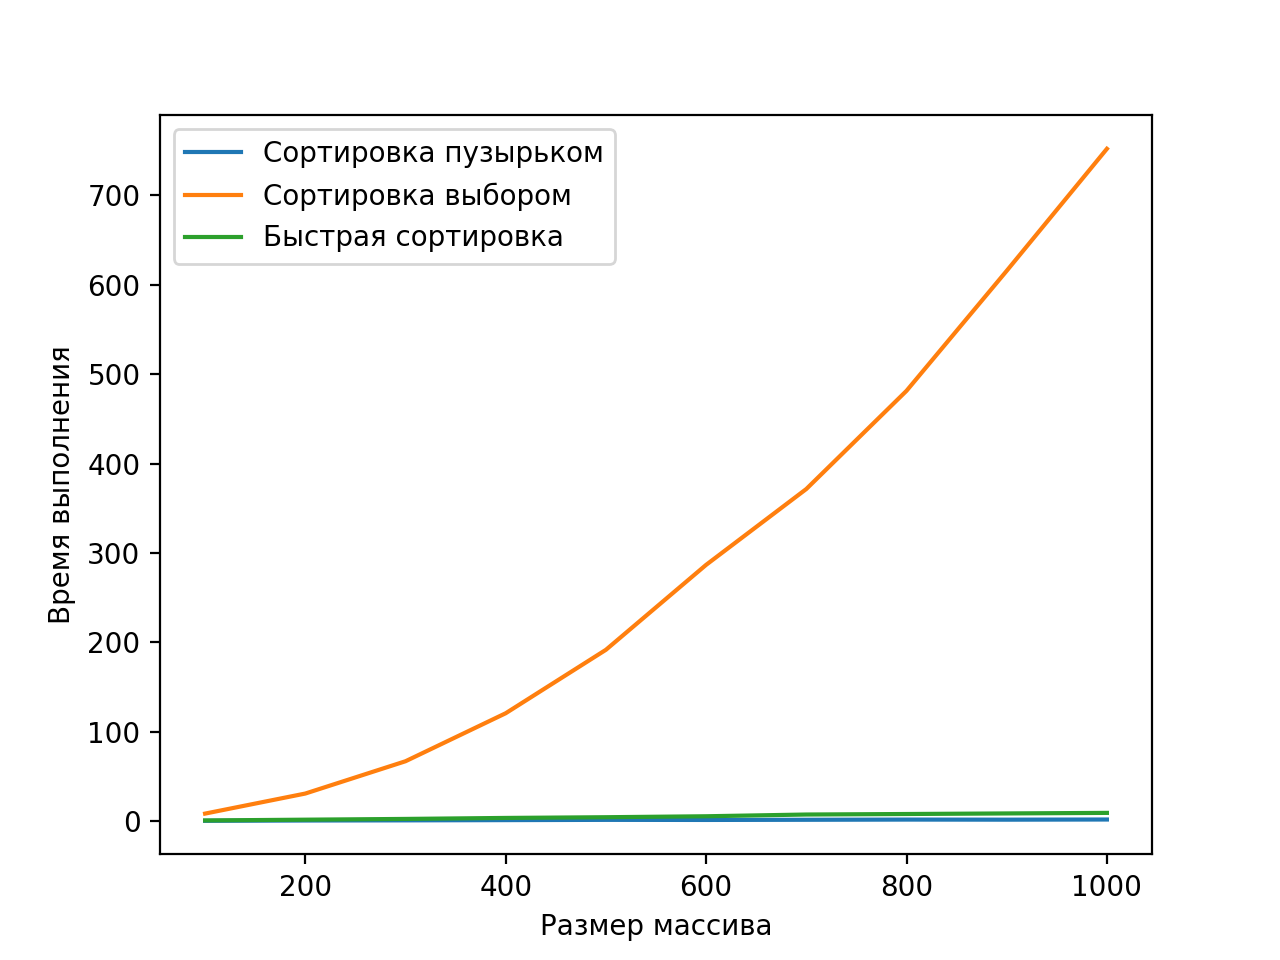
\includegraphics[scale = 0.8]{dir.png}
	\caption{Сортировки на отсортированных данных}
	\label{fig:mpr}
\end{figure}

\begin{figure}[h!p]
	\centering
	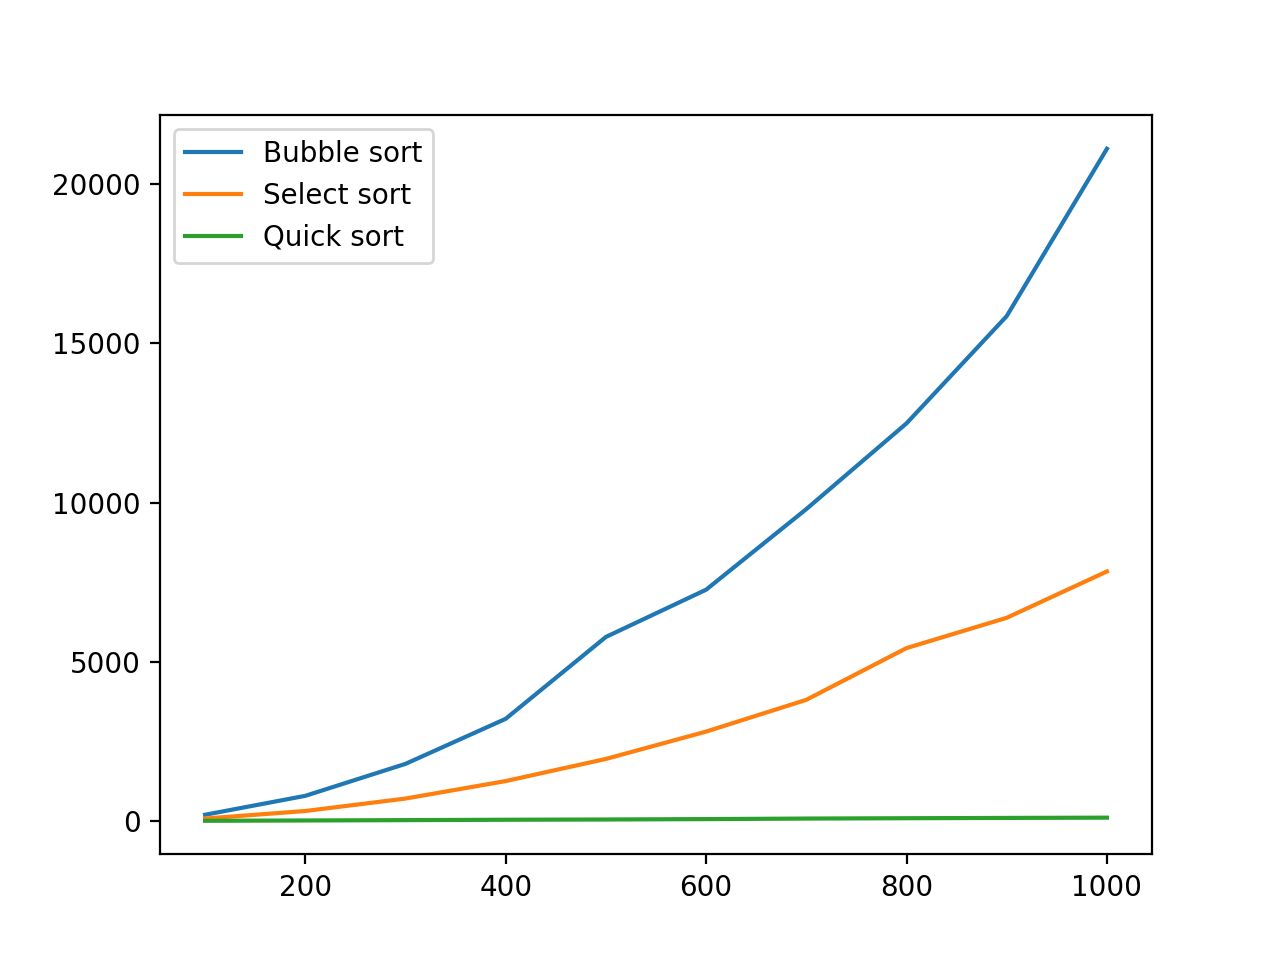
\includegraphics[scale = 0.8]{undir.png}
	\caption{Сортировки на отсортированных в обратном порядке данных}
	\label{fig:mpr}
\end{figure}

\begin{figure}[h!p]
	\centering
	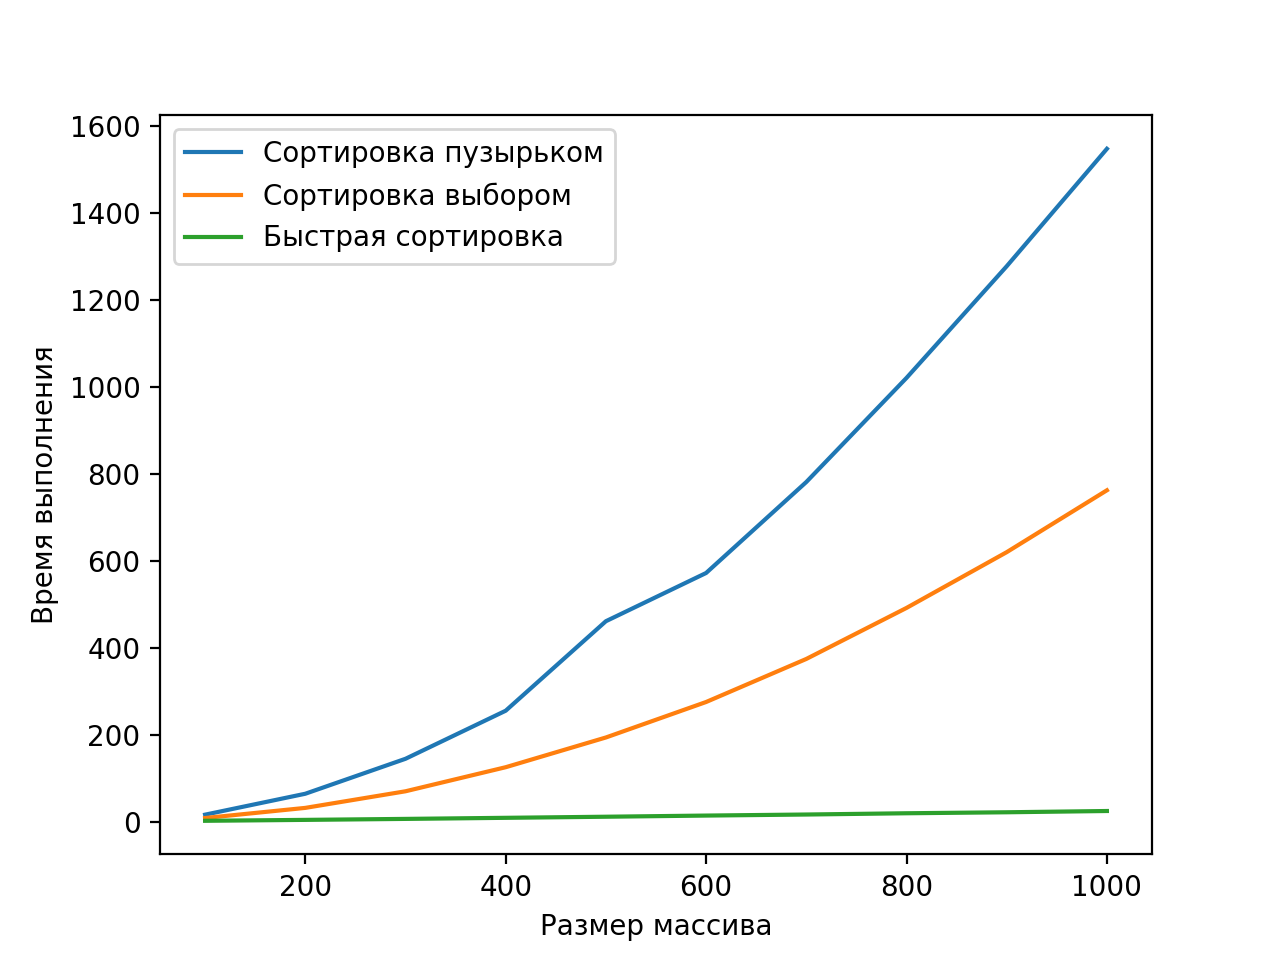
\includegraphics[scale = 0.8]{rand.png}
	\caption{Сортировки на произвольных данных}
	\label{fig:mpr}
\end{figure}

\begin{table} [h!]
	\caption{Таблица времени выполнения сортировок на отсортированных данных (в мс)}
	\begin{center}
	\begin{tabular}{|c c c c|}

		\hline

		Размер & bsort & ssort & qsort  \\ [0.5ex]

100 & 2.30 & 88.39 & 8.21  \\ 
\hline
200 & 3.65 & 330.28 & 19.30  \\ 
\hline
300 & 5.89 & 712.55 & 28.20  \\ 
\hline
400 & 6.95 & 1240.77 & 38.60  \\ 
\hline
500 & 8.20 & 1994.25 & 46.69  \\ 
\hline
600 & 11.26 & 2759.52 & 57.24  \\ 
\hline
700 & 11.50 & 3726.45 & 69.03  \\ 
\hline
800 & 12.59 & 4962.32 & 80.66  \\ 
\hline

	\hline 
	\end{tabular}
	\end{center}
\end{table}

\begin{table} [h!]
	\caption{Таблица времени выполнения сортировок на отсортированных данных в обратном порядке (в мс)}
	\begin{center}
	\begin{tabular}{|c c c c|}

		\hline

		Размер & bsort & ssort & qsort \\ [0.5ex]

100 & 210.89 & 81.22 & 9.19  \\ 
\hline
200 & 805.45 & 308.49 & 20.80  \\ 
\hline
300 & 1798.66 & 701.04 & 29.60  \\ 
\hline
400 & 3217.89 & 1642.31 & 91.78  \\ 
\hline
500 & 5283.90 & 1886.37 & 49.99  \\ 
\hline
600 & 7117.10 & 2815.29 & 65.26  \\ 
\hline
700 & 9821.45 & 3722.31 & 78.11  \\ 
\hline
800 & 12687.10 & 4902.62 & 89.13  \\ 
\hline

	\end{tabular}
	\end{center}
\end{table}

\begin{table} [h!]
	\caption{Таблица времени выполнения сортировок на случайных данных (в мс)}
	\begin{center}
	\begin{tabular}{|c c c c|}

		\hline

		Размер & bsort & ssort  & qsort \\ [0.5ex]
100 & 155.76 & 81.33 & 17.55  \\ 
\hline
200 & 608.76 & 308.62 & 40.25  \\ 
\hline
300 & 1397.26 & 697.15 & 65.97  \\ 
\hline
400 & 2490.49 & 1249.19 & 90.36  \\ 
\hline
500 & 4549.81 & 1868.65 & 107.29  \\ 
\hline
600 & 5471.37 & 2758.52 & 140.66  \\ 
\hline
700 & 8677.94 & 3838.68 & 162.69  \\ 
\hline
800 & 9923.00 & 4747.77 & 184.41  \\ 
\hline

	\end{tabular}
	\end{center}
\end{table}


\section{Вывод}

Как и ожидалось в результате оценки трудоемкости алгоритмов, сортировка пузырьком работает очень быстро на уже отсортированном массиве (лучший случай - оценка O(n)) и очень меделенно на отсортированном в обратном порядке (худший случай - оценка O($n^2$)). Время сортировки выбором на всех трёх видах массивов примерно одинаково, поскольку лучший и худший случаи работают за квадратичное время. Быстрая сортировка работает значительно лучше двух других сортировок во всех трёх приведённых случаях.


\chapter*{Заключение}
\addcontentsline{toc}{chapter}{Заключение}

В рамках данной лабораторной работы были решены следующие задачи:

\begin{itemize}
	\item изучены и реализованы 3 алгоритма сортировки: пузырьком, выбором, быстрая сортировка;
	\item протестированы реализованные алгоритмы;
	\item проведён сравнительный анализ трудоёмкости алгоритмов на основе теоретических расчетов;
	\item проведён сравнительный анализ алгоритмов по затраченному процессорному времени.
\end{itemize}

На основании анализа трудоемкости алгоритмов было показано, что алгоритм сортировки пузырьком имеет наименьшую сложность (линейную) в уже отсортированном массиве и квадратичную в отсортированном обратно, сортировка выбором имеет квадратичную сложность в лучшем, худшем и среднем случаях, а быстрая сортировка работает в лучшем и среднем случае значительно лучше (O(nlogn)) двух других алгоритмов, однако при неудачно выбранном опорном элементе и она может достигать квадратичной сложности. Те же выводы были подверждены экспериментально на основе замеров процессорного времени работы алгоритмов. 

\chapter*{Литература}
\addcontentsline{toc}{chapter}{Литература}
\begin{enumerate}
	\item Кормен Т. Алгоритмы: построение и анализ [Текст] / Кормен Т. - Вильямс, 2014. - 198 с. - 219 с.
	\item Стандартная функция clock(), измеряющая процессорное время [Электронный ресурс]. Режим доступа: https://en.cppreference.com/w/cpp/chrono/c/clock. Дата обращения: 17.09.2021
\end{enumerate}


\end{document}